\section{Experiments}

\subsection{Random Forest}
\subsubsection{Classification Performance with Varying Hyperparameters}
The key hyperparameters evaluated were the number of estimators and the maximum depth. The performance impact of varying these two parameters were primarily analyzed. The graph demonstrates that increasing both parameters leads to significant accuracy improvements up to a certain point, beyond which further increases result in diminishing returns.
\begin{figure}[!ht]
    \centering
    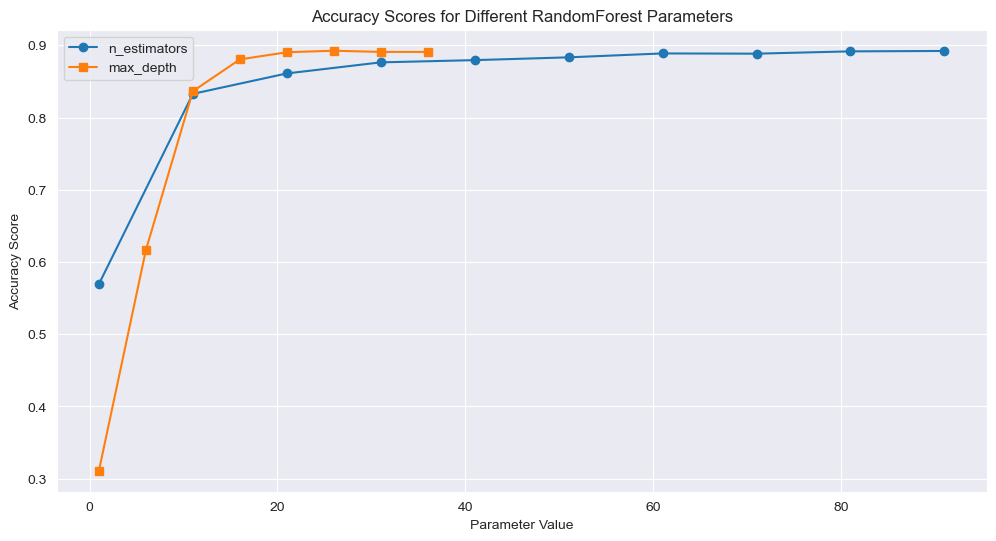
\includegraphics[scale=0.5]{fig/rfc_parameters.png}
    \vspace{-0.3cm}
    \caption{Performance on different hyperparameters}
    \label{fig:rfc_parameters}
    \vspace{-0.1cm}
\end{figure}

\subsubsection{Overfitting and Underfitting Analysis}
Overfitting was particularly evident when using high numbers of estimators, but this was mitigated by visualizing the accuracy across different numbers of estimators and adjusting the parameter accordingly based on the plot.
The training score remained consistently at 1.0 or 100\% across all sample sizes, indicating that the model perfectly fit the training data. This perfect score, however, suggests that the model was likely overfitting. In contrast, the cross-validation score started at approximately 75\% with smaller sample sizes and gradually increased to about 90\% as the sample size grew. This improvement indicates that the model's ability to generalize to unseen data improved with more training samples, thereby reducing overfitting.

\begin{figure}[!ht]
    \centering
    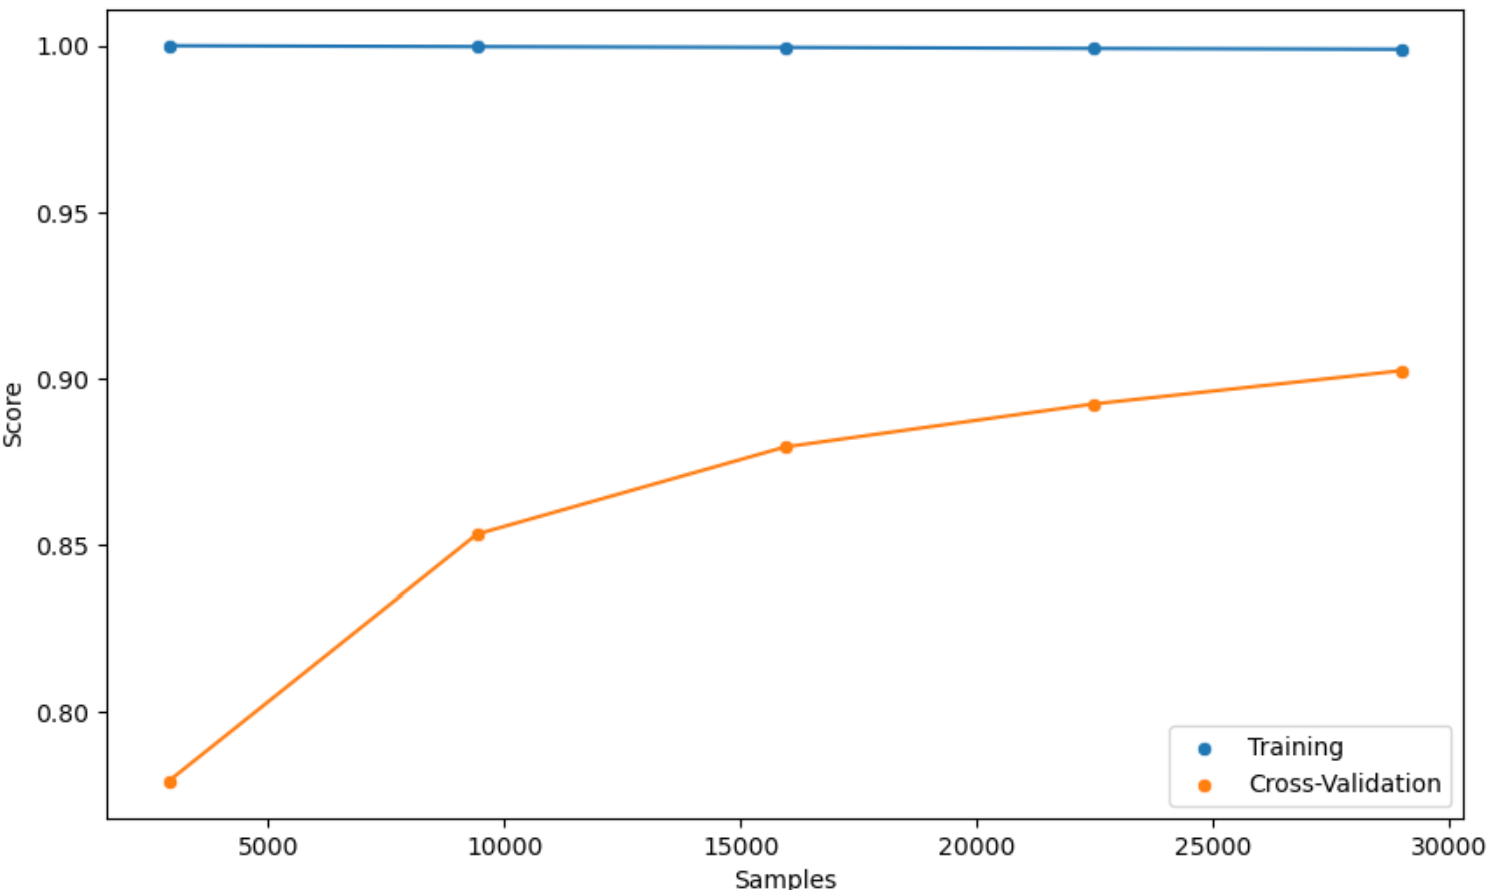
\includegraphics[scale=0.5]{fig/rfc_learning_curve.png}
    \vspace{-0.3cm}
    \caption{Learning Curve}
    \label{fig:rfc_learning_curve}
    \vspace{-0.1cm}
\end{figure}

\subsubsection{Final Unbiased Performance Comparison}
Overall, the Random Forest model demonstrates robust performance in classifying the speech data, with particularly high accuracy and well-balanced precision and recall across most categories. The exceptions that did not perform as well were expected, as words like "Ofen," "offen," "Licht," and "nicht" are pronounced quite similarly.

\begin{table}
  \caption{Classification Report for Random Forest Model}
  \label{tab:classification_report}
  \centering
  \begin{tabular}{lccc}
    \toprule
    Class        & Precision & Recall & F1-score \\
    \midrule
    Alarm        & 0.93 & 0.91 & 0.92 \\
    Command an   & 0.91 & 0.87 & 0.89 \\
    Command aus  & 0.89 & 0.86 & 0.87 \\
    Fernseher    & 0.98 & 0.88 & 0.93 \\
    Heizung      & 0.99 & 0.89 & 0.94 \\
    Licht        & 0.93 & 0.82 & 0.87 \\
    Lüftung      & 0.98 & 0.93 & 0.95 \\
    Miscellaneous & 0.89 & 0.96 & 0.92 \\
    Objects      & 0.90 & 0.96 & 0.93 \\
    Ofen         & 0.82 & 0.70 & 0.76 \\
    Radio        & 0.99 & 0.88 & 0.93 \\
    Status       & 0.84 & 0.86 & 0.85 \\
    Staubsauger  & 0.99 & 0.90 & 0.94 \\
    \midrule
    Accuracy     & \multicolumn{3}{c}{0.91} \\
    \bottomrule
  \end{tabular}
\end{table}

\subsection{Nearest Neighbour}
\subsubsection{Classification Performance with Varying Hyperparameters}
Present the results of experiments with different hyperparameter values. Visualize the change in performance.
\subsubsection{Overfitting and Underfitting Analysis}
Discuss the extent of overfitting or underfitting observed. Explain how these issues depend on hyperparameter values.
\subsubsection{Final Unbiased Performance Comparison}
Summarize the results in a comparative table or plot.

\subsection{CNN}
\subsubsection{Classification Performance with Varying Hyperparameters}
The CNN architecture was tested with various hyperparameters, including the number of filters, kernel sizes, and dropout rates. The key hyperparameters evaluated were:
\begin{itemize}
    \item \textbf{Number of Filters}: Tested configurations included 8, 16, 32, and 64 filters in different layers.
    \item \textbf{Kernel Sizes}: Kernel sizes of 7, 9, 11, and 13 were tested to determine the optimal receptive field.
    \item \textbf{Dropout Rates}: Dropout rates of 0.3, 0.4, and 0.5 were evaluated to prevent overfitting.
\end{itemize}
The results showed that increasing the number of filters and adjusting the kernel sizes provided a balance between model complexity and performance, with optimal configurations leading to improved accuracy and generalization.

\subsubsection{Overfitting and Underfitting Analysis}
The CNN model showed signs of overfitting at higher dropout rates and excessive numbers of filters. This was evident from the gap between training and validation accuracy. By adjusting these hyperparameters, overfitting was mitigated. The training and validation accuracy curves indicated that the model generalized well with a balanced configuration of filters and dropout rates.

\begin{figure}[!ht]
    \centering
    \includegraphics[scale=0.5]{fig/cnn_hyperparameters.png}
    \vspace{-0.3cm}
    \caption{CNN Performance with Varying Hyperparameters}
    \label{fig:cnn_hyperparameters}
    \vspace{-0.1cm}
\end{figure}

\begin{figure}[!ht]
    \centering
    \includegraphics[scale=0.5]{fig/cnn_learning_curve.png}
    \vspace{-0.3cm}
    \caption{CNN Learning Curve}
    \label{fig:cnn_learning_curve}
    \vspace{-0.1cm}
\end{figure}

\subsubsection{Final Unbiased Performance Comparison}
The CNN model achieved the following final performance metrics on the test set:
\begin{itemize}
    \item \textbf{Accuracy}: 92.26\%
    \item \textbf{Precision}: 92.75\%
    \item \textbf{Recall}: 92.28\%
    \item \textbf{F1-score}: 92.21\%
\end{itemize}

Overall, the CNN model demonstrated superior performance compared to the Random Forest and Nearest Neighbour classifiers, particularly in terms of accuracy and generalization across different categories.

\begin{table}
  \caption{Classification Report for CNN Model}
  \label{tab:cnn_classification_report}
  \centering
  \begin{tabular}{lcccc}
    \toprule
    Class        & Precision & Recall & F1-score & Support \\
    \midrule
    Alarm        & 0.91 & 0.99 & 0.95 & 294 \\
    Brötchen     & 0.96 & 0.93 & 0.94 & 308 \\
    Fernseher    & 0.94 & 0.97 & 0.95 & 306 \\
    Haus         & 0.91 & 0.96 & 0.93 & 329 \\
    Heizung      & 0.97 & 0.96 & 0.97 & 310 \\
    Leitung      & 0.96 & 0.96 & 0.96 & 321 \\
    Licht        & 0.72 & 0.95 & 0.82 & 280 \\
    Lüftung      & 0.94 & 0.97 & 0.96 & 297 \\
    Ofen         & 0.72 & 0.89 & 0.79 & 319 \\
    Radio        & 0.96 & 0.98 & 0.97 & 302 \\
    Schraube     & 0.98 & 0.97 & 0.97 & 317 \\
    Spiegel      & 0.98 & 0.98 & 0.98 & 283 \\
    Staubsauger  & 0.99 & 0.95 & 0.97 & 319 \\
    an           & 0.91 & 0.92 & 0.92 & 328 \\
    aus          & 0.94 & 0.89 & 0.92 & 297 \\
    kann         & 0.93 & 0.90 & 0.91 & 314 \\
    nicht        & 0.92 & 0.66 & 0.77 & 304 \\
    offen        & 0.86 & 0.62 & 0.72 & 282 \\
    other        & 0.98 & 0.95 & 0.97 & 680 \\
    warm         & 0.96 & 0.94 & 0.95 & 321 \\
    wunderbar    & 0.98 & 0.99 & 0.98 & 281 \\
    \midrule
    Accuracy     & \multicolumn{4}{c}{0.92} & 6792 \\
    Macro avg    & 0.92 & 0.92 & 0.92 & 6792 \\
    Weighted avg & 0.93 & 0.92 & 0.92 & 6792 \\
    \bottomrule
  \end{tabular}
\end{table}
